\begin{figure}[h!]
\tikzset{every picture/.style={line width=0.75pt}} %set default line width to 0.75pt        
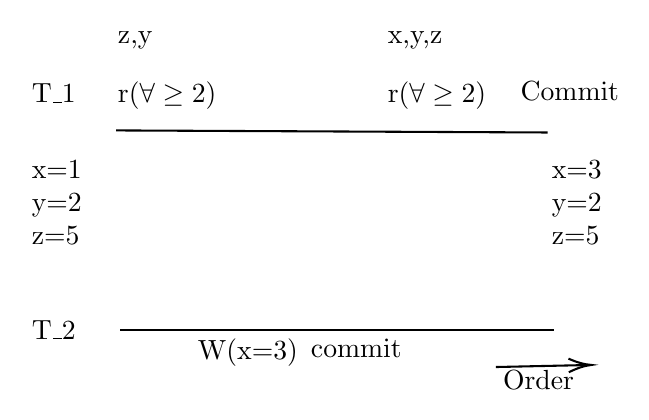
\begin{tikzpicture}[x=0.75pt,y=0.75pt,yscale=-1,xscale=1]
%uncomment if require: \path (0,300); %set diagram left start at 0, and has height of 300

%Straight Lines [id:da9500410641573396] 
\draw    (63.56,64) -- (271.56,65) ;
%Straight Lines [id:da7796185686481738] 
\draw    (65.56,160) -- (274.56,160) ;
%Straight Lines [id:da7329480179958066] 
\draw    (246.56,178) -- (290.56,177.04) ;
\draw [shift={(292.56,177)}, rotate = 178.75] [color={rgb, 255:red, 0; green, 0; blue, 0 }  ][line width=0.75]    (10.93,-3.29) .. controls (6.95,-1.4) and (3.31,-0.3) .. (0,0) .. controls (3.31,0.3) and (6.95,1.4) .. (10.93,3.29)   ;

% Text Node
\draw (21.5,40) node [anchor=north west][inner sep=0.75pt]   [align=left] {T\_1};
% Text Node
\draw (21.5,154) node [anchor=north west][inner sep=0.75pt]   [align=left] {T\_2};
% Text Node
\draw (101.56,163) node [anchor=north west][inner sep=0.75pt]   [align=left] {W(x=3)};
% Text Node
\draw (63,39) node [anchor=north west][inner sep=0.75pt]   [align=left] {r($\forall \geq 2$)};
% Text Node
\draw (257,39) node [anchor=north west][inner sep=0.75pt]   [align=left] {Commit};
% Text Node
\draw (156,163) node [anchor=north west][inner sep=0.75pt]   [align=left] {commit};
% Text Node
\draw (248.56,178) node [anchor=north west][inner sep=0.75pt]   [align=left] {Order};
% Text Node
\draw (21.5,77) node [anchor=north west][inner sep=0.75pt]   [align=left] {x=1\\y=2\\z=5};
% Text Node
\draw (193,15) node [anchor=north west][inner sep=0.75pt]   [align=left] {x,y,z};
% Text Node
\draw (63,15) node [anchor=north west][inner sep=0.75pt]   [align=left] {z,y};
% Text Node
\draw (193,39) node [anchor=north west][inner sep=0.75pt]   [align=left] {r($\forall \geq 2$)};
% Text Node
\draw (272,77) node [anchor=north west][inner sep=0.75pt]   [align=left] {x=3\\y=2\\z=5};

\end{tikzpicture}
\caption{P3: Phantom Read $T_1$ and $T_2$}
\end{figure}